% The main file for TUM reports

\documentclass[11pt,                % font size
               a4paper,             % paper size
               oneside,             % one sided
               listof=totoc,        % add lists of figures and tables to toc
               bibliography=totoc,  % add bibliography to toc
               index=totoc,         % add index to toc
               headsepline,         % add a separation line between head and content
               footsepline,         % add a separation line between foot and content
               plainfootsepline,    % add a foot line on chapter pages
               footinclude=false,   % determine whether the page footer are considered as part
               headinclude=true,    % of the page body for the calculation of the type area.
               BCOR12mm,            % binding correction
               numbers=noenddot,    % use Figure x.y: i.o. Figure x.y.:
               draft,               % show badboxes and hide graphics
              ]{scrbook}

% Set here the title, authors and other stuff to be used for the cover

\def\doctype{Bachelorarbeit in Informatik}
\def\title{On the new threats of social engineering exploiting social networks}
\def\titleGer{Neue Bedrohungen bei Sozialen Netzwerken im Bezug auf Social Engineering}
\def\author{Daniel Siegel}
\def\date{August 15, 2009}

% text to appear in the footer
\def\footertext{}

\usepackage{scrpage2}

\usepackage[utf8]{inputenc}
\usepackage[T1]{fontenc}
\usepackage[ngerman,english]{babel}
\usepackage{cmbright}

\usepackage[pdftex]{graphicx}
\usepackage{ifthen}
\usepackage{subfigure}
\usepackage{colortbl}
\usepackage{multirow}
\usepackage{url}
\usepackage{color}
\usepackage{makeidx}
\usepackage{float}
\usepackage{rotating}

\usepackage{styles/tumlogo}
\usepackage{styles/shortoverview}
\usepackage{styles/secnum}
\usepackage[Sonny]{styles/myfncychap}

\usepackage[pdftex,colorlinks=true,linkcolor=red,citecolor=red,%
anchorcolor=red,urlcolor=red,bookmarks=true,%
bookmarksopen=true,bookmarksopenlevel=0,plainpages=false%
bookmarksnumbered=true,hyperindex=false,pdfstartview=%
]{hyperref}

%% mark text as preliminary
\usepackage[draft,german,scrtime]{prelim2e}

\usepackage{scrpage2}
\pagestyle{scrheadings}
\ifoot[\footertext]{\footertext} % \footertext set in INFO.TEX

\usepackage[utf8]{inputenc}
\usepackage[T1]{fontenc}
\usepackage[ngerman,english]{babel}
\selectlanguage{english}

\usepackage[pdftex]{graphicx}
\graphicspath{{figures/}}

\usepackage{cmbright}

\usepackage{ifthen}
\usepackage{subfigure}
\usepackage{colortbl}
\usepackage{multirow}
\usepackage{url}
\usepackage{color}
\usepackage{makeidx}
\usepackage{float}
\usepackage{rotating}

\usepackage{styles/tumlogo}
\usepackage{styles/shortoverview}
\usepackage{styles/secnum}


\usepackage[pdftex,colorlinks=true,linkcolor=red,citecolor=red,%
anchorcolor=red,urlcolor=red,bookmarks=true,%
bookmarksopen=true,bookmarksopenlevel=0,plainpages=false%
bookmarksnumbered=true,hyperindex=false,pdfstartview=%
]{hyperref}

\hypersetup{%
  pdftitle    = \title,
  pdfsubject  = {Bachelor thesis},
  pdfauthor   = {Daniel Siegel},
  colorlinks  = true,
  linkcolor   = blue,
  urlcolor    = red,
  breaklinks  = true,
}


%% Fancy chapters

% set the bibliography style
\bibliographystyle{styles/bauermaNum}
%\bibliographystyle{alpha}
%\bibliographystyle{plain}

% Disable single lines at the start of a paragraph (Schusterjungen)
% Disable single lines at the end of a paragraph (Hurenkinder)
\clubpenalty = 10000
\widowpenalty = 10000
\displaywidowpenalty = 10000

%% mark text as preliminary
\usepackage[draft,german,scrtime]{prelim2e}

% Commands to be used within the TUM report document

% comment that appears on the border - very practical !!!
\newcommand{\comment}[1]{\marginpar{\raggedright \noindent \footnotesize {\sl #1} }}

% page clearing
\newcommand{\clearemptydoublepage}{%
  \ifthenelse{\boolean{@twoside}}{\newpage{\pagestyle{empty}\cleardoublepage}}%
  {\clearpage}}


\newcommand{\Twitter}{{\em{Twitter}}}


\begin{document}

  \frontmatter

  % The front cover for the TUM report document.

% correct BCOR - undo at the end !!!
\def\bcorcor{0.15cm}
\addtolength{\hoffset}{\bcorcor}

\thispagestyle{empty}

 \vspace{4cm}
\begin{center}
  \oTUM{4cm}

  \vspace{5mm}     
  \huge FAKULT{\"A}T F{\"U}R INFORMATIK\\ 
  \vspace{0.5cm}
  \large DER TECHNISCHEN UNIVERSIT{\"A}T M{\"U}NCHEN\\
  \vspace{1mm}

\end{center}

\vspace{15mm}
\begin{center}

  {\Large \doctype}
  \vspace{20mm}

  {\huge\bf \title}\\%[3ex]
  \vspace{15mm}

  {\LARGE  \author}
  \vspace{10mm}

  \begin{figure}[h!]
  \centering
   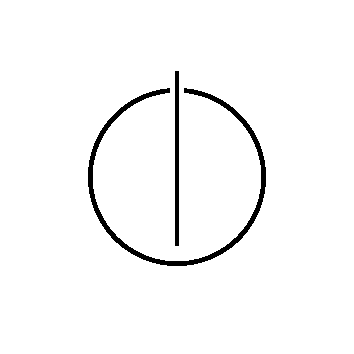
\includegraphics[width=4cm]{styles/informat.png}
  \end{figure}

\end{center}


  \clearemptydoublepage

  % The titlepage for the CAMP report document.

%--------------------------------------------------
% The title page
%--------------------------------------------------

\thispagestyle{empty}

\vspace{10mm}

\begin{center}
  \oTUM{4cm}

  \vspace{5mm}
  \huge FAKULTÄT FÜR INFORMATIK\\
  \vspace{0.5cm}
  \large DER TECHNISCHEN UNIVERSITÄT MÜNCHEN\\
  \vspace{1mm}
\end{center}

\vspace{10mm}
\begin{center}
  {\Large \doctype}
  \vspace{10mm}

  {\LARGE \textbf \title}\\
  \vspace{10mm}

  {\LARGE \textbf \titleGer}\\
  \vspace{10mm}

  \begin{tabular}{ll}
    \Large Author:     & \Large \author \\[2mm]
    \Large Supervisor: & \Large Univ.-Prof. Dr. Claudia Eckert \\[2mm]
    \Large Advisor:    & \Large Dipl.Inf. Werner Streitberger\\[2mm]
    \Large Date:       & \Large August 15, 2009
  \end{tabular}

  \vspace{5mm}

  \begin{figure}[h!]
  \centering
  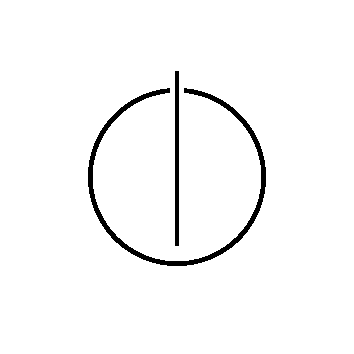
\includegraphics[width=4cm]{styles/informat.png}
  \end{figure}
\end{center}


  \clearemptydoublepage

\thispagestyle{empty}
\selectlanguage{ngerman}
  \vspace*{0.8\textheight}
  \noindent
  Ich versichere, dass ich diese Bachelorarbeit selbstständig verfasst und nur\\
  die angegebenen Quellen und Hilfsmittel verwendet habe.

  \vspace{15mm}
  \noindent
  M{\"u}nchen, den \today \hspace{5cm} \author
\selectlanguage{english}
\newpage


%  \clearemptydoublepage
\phantomsection
\addcontentsline{toc}{chapter}{Acknowledgements}	

\vspace*{2cm}

\begin{center}
{\Large \bf Acknowledgments}
\end{center}

\vspace{1cm}

If someone contributed to the thesis... might be good to thank them here.


  % Abstract for the TUM report document
% Included by MAIN.TEX


\clearemptydoublepage
\phantomsection
\addcontentsline{toc}{chapter}{Abstract}	





\vspace*{2cm}
\begin{center}
{\Large \bf Abstract}
\end{center}
\vspace{1cm}

An abstracts abstracts the thesis!

  \tableofcontents
  \enlargethispage{1.05\baselineskip}

  \mainmatter

  \chapter{Introduction}
\label{chapter:introduction}

\section{Problem and Motivation}

Social Networks, such as Facebook\footnote{\url{http://www.facebook.com}},
MySpace\footnote{\url{http://www.myspace.com}} or
Twitter\footnote{\url{http://www.twitter.com}} gained million of members on
their platforms in the last years. They are widely used in both private and
business networking. Services, like the one just mentioned, allow individuals
to present their own identity and to share and keep relationships to other
members of those services. Often, they are also presenting their information to
an unknown number of strangers.

This brings us not only to the question how useful a social network is for a
single user, but also if there are any drawbacks or risks.  Users often put
much and frequently sensitive data into their profiles, as for example
\cite{brown2008} shows.  This data however is stored centrally at the company
which provides the network and so the user looses the control over his
data~\cite{fraunhofer2008}.

There is of course a relation between the data the user entered and the user
himself. Following that thought, another person is not only able to extract the
data but also to obtain new information or rather interpretations, which were
not entered by the user.

Many studies, like \cite{fraunhofer2008,gross2005} show already, that this can
be a massive intervention into one's privacy. This work however wants to examine
whether such information are a security risk and can be used for attacks
against a company or an individual.

Of course, a distinction between employees of a certain company and private
users has to be made. For example, certain information can be harmless to an
individual, but very well a danger to a company \cite{mitnick2003}. In both
cases, however, a social engineer saves an additional step, for example a
telephone call or similar, to get that specific information. That step does not
only require extra work, but also the danger of being exposed. Without his
anonymity, a social engineer could not carry out an attack \cite{mitnick2003}.

Especially in big corporations spend hundreds of thousands or dollars for the
security of their IT-infrastructure. An attack at the IT-layer would therefore
often be very laborious. Therefore it is much simpler bypass the security
mechanisms through social engineering, as it very cheap and does not require
any superior technology \cite{winkler1995}. Commonly, a skilled social
engineering does not require anything more than a telephone for such attacks
\cite{mitnick2003}.

Concretely, this study wants to answer the following questioning:
How can data of individuals or companies automatically be extracted
from social networks and presented in a way, that it can be used for a social
engineering attack. In addition, countermeasures against automatic extraction
and social engineering attacks are going to be developed.

\section{Outline of the thesis}

\noindent {\textbf{Chapter 1}: Introduction}
\vspace{0.5em}\\
\noindent This chapter presents an overview of the thesis and it's purpose.
%Furthermore, it will discuss the threats and risks of social engineering and
%contain a glossary.

\noindent {\textbf{Chapter 2}: Related Work}
\vspace{0.5em}\\
\noindent The section will outline related works in the field of social
engineering, the attacks and countermeasures. It will present common attacks
and how companies and individuals can protect themselves against such attacks.

\noindent {\textbf{Chapter 3}: Analysis of the social network \Twitter}
\vspace{0.5em}\\
\noindent The study takes a deeper look at the social network \Twitter. It will
show the drawbacks and risks of such social networks, the data, which can be
extracted automatically, how sample attacks could look like and finally the
countermeasures against such attacks.

\noindent {\textbf{Chapter 4}: Design, analysis and implementation of a prototype}
\vspace{0.5em}\\
\noindent In this chapter, a prototype, who automatically can harvest data and
present it in a way, that it can be used for social engineering attacks, is
developed. The usual software engineering methods are used.

\noindent {\textbf{Chapter 5}: Evaluation}
\vspace{0.5em}\\
\noindent This chapter wants to examine, whether the already described attacks
can be achieved by using the prototype and therefore shows a sample attack. It
will analyse the attack and evaluate the risk against a company or an
individual.

\noindent {\textbf{Chapter 6}: Conclusion}
\vspace{0.5em}\\
\noindent The thesis finally concludes draws together the main findings of the
study.

\section{Glossary}


  \chapter{Related Work}
\label{chapter:relatedwork}


\section{Mögliche Social Engineering Angriffe}
\subsection{\glqq{}Digitale\grqq{} Angriffe}
\subsubsection{Phishing}
\subsubsection{Baiting}
\subsubsection{\dots}
\subsection{\glqq{}Analoge\grqq{} Angriffe}
\subsubsection{Pretexting}
\subsubsection{Identitätsdiebstahl}
\subsubsection{\dots}
\section{Schutzmöglichkeiten vor Social Engineering Angriffen bei
Privatpersonen und Unternehmen}
\subsection{Awareness}
\subsection{Unternehmens-Policy}
\subsection{Abschottung von Informationen}
\subsection{Schulung der Mitarbeiter}
\subsection{Technische Schutzmöglichkeiten}
\subsection{\dots}


  \chapter{Selection of Social Engineering Attacks}
\label{chap:attacks}

The previous chapter showed already sample social engineering attacks, the
threats it exposes and their countermeasures. The work wants to assign now selected
social engineering attacks to social networks and find out, what new threats
they disclose. Furthermore, the attacks should constitute a part of the demand
of the prototype, which will be developed.

All of the following attacks are described by Mitnick and Simon
\cite{mitnick2003} and happened in the past.

\section[Phishing mail]{Phishing mail (\cite[pp. 97-100]{mitnick2003})}
\label{sec:phishing_mail}

The first attack is an attack against a private person, with no affiliation at
a company. A phishing mail is used to trick the victim into revealing his
username and password of an online payment service. A definition of the term
\textit{phishing} is as follows~\cite{jagatic2007}:

\begin{quote}
\textit{Phishing is a form of deception in which an attacker attempts to
fraudulently acquire sensitive information from a victim by impersonating a
trustworthy entity. Phishing attacks typically employ generic
\glqq{}lures\grqq{}.}
\end{quote}

The enormous threat, phishing attacks can present, was already shown in section
\ref{subsection:active_attacks}. The following scenario was therefore chosen
because of it's relevancy and the fact, that just individuals are being
attacked.

The victim, a retired insurance salesman named Edgar, received an e-mail from
\textit{PayPal}\footnote{\url{http://www.paypal.com}}, which is a company that
offers a fast and secure way to make online payments. Edgar did use
\textit{PayPal} often, as he was a collector of antique glass jars. Therefore
he used the service several times a week. The e-mail he received during the
holiday season 2001 was looking officially from \textit{PayPal}, offering him a
requital for updating his \textit{PayPal} account. The message looked like the
following~\cite[p. 97]{mitnick2003}:

\begin{quote}
Season's Greetings Valued PayPal Customer;

As the New Year approaches and as we all get ready to move a year ahead,
PayPal would like to give you a \$5 credit to your account!

All you have to do to claim your \$5 gift from us is update your information on
our secure Pay Pal site by January 1st, 2002. A year brings a lot of changes,
by updating your information with us you will allow for us to continue
providing you and our valued customer service with excellent service and in the
meantime, keep our records straight! To update your information now and to
receive \$5 in your PayPal account instantly, click this link:

\url{http://www.paypal-secure.com/cgi-bin}

Thank you for using PayPal.com and helping us grow to be the largest of our
kind!

Sincerely wishing you a very "Merry Christmas and Happy New Year,"

PayPal Team

\end{quote}

One might notice several signs in the message, that can lead to the belief,
that something is wrong with the e-mail. For example, the semicolon after the
greeting line, the blemished text about 
\glqq{}our valued customer service with excellent service and in the\grqq{} and
most noticeable the URL, which does not lead to \url{http://www.paypal.com} but
to a different domain. Edgar clicked on the link, entered the information
requested, which was name, address, phone number and credit card number. He
then was waiting for the \$5 gift to show up, but what showed up was a list of
charges he never purchased on his credit card bill.

The victim is not a single one, there are many scams which look like the above.
The attack was also prepared properly, as they knew that Edgar was a PayPal
customer. If he would not have been, the attack certainly wouldn't have worked.

To make the attack even more realistic and effective, the message could have also
been sent to the victim's friends and colleagues, if they are also a member of
the same electronic payment service.

\begin{table*}[ht]
  \centering
  \ra{1.3}
  \begin{tabular}{p{0.8\textwidth}c}
    \toprule
    Information & Required\\
    \midrule
    Real name & \checkmark\\
    E-mail address & \checkmark\\
    Knowledge of account of an electronic payment service & \checkmark\\
    E-mail addresses of friends and colleagues & \\
    Knowledge, which friend or colleague has an account on an electronic
    payment service & \\
    \bottomrule
  \end{tabular}
  \caption{Overview of the required data of the phishing attack.}
\end{table*}

\section[Insider attack]{Insider attack (\cite[pp. 83-89]{mitnick2003})}
\label{sec:insider_attack}

Another real case scenario was an attack, which involved stealing source code
from a company containing the encryption algorithms and firmware used in the
company radio products. It's relevance is the fact, that this was an attack
against a company, involving information gathering about the company structure,
security devices used inside the company and having several employees as
victims. Due to it's manifold character, this attack could be extended to
similar attacks, which even could require less information.

The attacker, called \textit{Danny} by Mitnick, began his information retrieval
on the Internet. He luckily found a years-old message written by an employee of
the affected company and posted to a public readable newsgroup. This message
contained a signature including the employee's name, his phone number and
workgroup. He now had to check if that person still works for that company. He
called the employee, who indeed was still working for the same company, and
manipulated him to reveal the names of the servers, the employees used for
development work.

In addition, every employee in the company had a small electronic device called
\textit{Secure ID} in addition to their username and password. The attacker
managed to get enough pieces of information about the company together to
masquerade as a real employee. He now had an employee's name, residence
address, phone number, department and employee number, the manager's name and
phone number. Furthermore he knew the servers he needed access for.

Danny now waited for a snow storm in the location of the employee's residence.
As it was winter, he did not have to wait very long and he launched the attack.
He telephoned the IT department and talked to a computer operator named Roger
Kowalski.

The attack went as follows~\cite[p. 86]{mitnick2003}:

\begin{quote}
\textit{Danny:} \glqq{}This is Bob Billings. I work in the Secure Communications Group. I'm at
home right now and I can't drive in because of the storm. And the problem is
that I need to access my workstation and the server from home, and I left my
Secure ID in my desk. Can you go fetch it for me? Or can somebody? And then
read off my code when I need to get in? Because my team has a critical deadline
and there's no way I can get my work done. And there's no way I can get to the
office--the roads are much too dangerous up my way.\grqq{}\\
\textit{Roger Kowalski:} \glqq{}I can't leave the Computer Center.\grqq{}\\
\textit{Danny:} \glqq{}Do you have a Secure ID yourself?.\grqq{}\\
\textit{Roger Kowalski:} \glqq{}There's one here in the Computer Center, we keep one
for the operators in case of an emergency.\grqq{}\\
\textit{Danny:} \glqq{}Listen, can you do me a big favor? When I need to dial into
the network, can you let me borrow your Secure ID? Just until it's safe to
drive in.\grqq{}\\
\textit{Roger Kowalski:} \glqq{}Who are you again? Who do you work for.\grqq{}\\
\textit{Danny:} \glqq{}For Ed Trenton.\grqq{}\\
\textit{Roger Kowalski:} \glqq{}Oh, yeah, I know him.\grqq{}\\
\textit{Danny:} \glqq{}I'm on the second floor, next to Roy Tucker.\grqq{}\\

\end{quote}

The operator of course was uncomfortable walking into the office desk and
looking through foreign property. But he was uncomfortable not helping either,
so he asked his manager and actually vouched for the attacker. The manager
wanted to speak to the attacker personally and the operator gave him the name
and phone number.

\begin{table*}[h]
  \centering
  \ra{1.3}
  \begin{tabular}{p{0.8\textwidth}c}
    \toprule
    Information & Required\\
    \midrule
    \multicolumn{2}{l}{Colleagues}\\
    \hspace{0.5cm} Name & \checkmark\\
    \hspace{0.5cm} Phone number & \checkmark\\
    \hspace{0.5cm} Department & \checkmark\\
    \hspace{0.5cm} Employee number & \\
    \multicolumn{2}{l}{Manager}\\
    \hspace{0.5cm} Name & \checkmark\\
    \hspace{0.5cm} Phone number & \\
    Residence of an employee & \checkmark\\
    Weather information & \checkmark\\
    Company and employee structure & \checkmark\\
    The knowledge, what security devices were used in the company & \checkmark\\
    The servers names and location & \checkmark\\
    \bottomrule
  \end{tabular}
  \caption{Overview of the required data of the insider attack.}
\end{table*}

The attacker then called the manager and explained the same story again,
mentioning that his team has a critical deadline. The manager then allowed him
to use the \textit{Secure ID} device in the IT department just for the weekend.
From now on, Danny just needed to call in and ask the operators to pass him the
\textit{Secure ID} token. Furthermore he was able to get a temporary account to
bypass the firewall restrictions, directly from the operator. Now, he had the
whole weekend to find a security hole which he found.

\section{The bank heist}
\label{sec:bank_heist}

The last attack was chosen, due to the fact, that it uses information, which is
not available on any social networks or the Internet. Again, this is an attack
against a company, including information about several employees, the company
structure and the already mentioned secret information.

\begin{table*}[ht]
  \centering
  \ra{1.3}
  \begin{tabular}{p{0.8\textwidth}c}
    \toprule
    Information & Required\\
    \midrule
    \multicolumn{2}{l}{Employee of the wire transfer room}\\
    \hspace{0.5cm} Name & \checkmark\\
    \hspace{0.5cm} Employee number & \checkmark\\
    \multicolumn{2}{l}{Employee outside the wire transfer room}\\
    \hspace{0.5cm} Name & \checkmark\\
    \hspace{0.5cm} Department & \checkmark\\
    \hspace{0.5cm} Employee number & \checkmark\\
    Phone number of wire transfer room & \checkmark\\
    Current wire transfer code & \checkmark\\
    \bottomrule
  \end{tabular}
  \caption{Overview of the required data of the phishing attack.}
\end{table*}

The bank heist was executed in 1978 by Stanley Mark Rifkin. It was the largest bank
robbery in U.S. history by that time. He stole 10.2 million U.S. dollars
through wire transfer just by using a telephone and social engineering
techniques.

Rifkin was working for a company under contract developing a backup system for
the Security Pacific National Bank and more specific for the wire transfer
system. As he was working inside the wire transfer room, he had the possibility
to learn the process of bank wire transfer. As the bank changed the
required transfer code daily, most employees did write the code down in order
to not have to memorize it every day. He then tried to adept the names, room
numbers and employee numbers. One day he additionally memorized the daily code and
executed a wire transfer over a callbox outside of the bank. Rifkin transfered
over 10 million U.S. dollars to a bank in Switzerland by just using the
information he already had gained and social engineering techniques.

He then picked up the money in Switzerland, changed it into diamonds and flew
back to the United States. As he tried to sell them there, the FBI quickly
captured him.


  \chapter{Analysis of the social network \Twitter}
\label{chapter:analysis}

\section{Reasons for choosing this social network}

\section{Threats and risks}

\section{Relevant data and the security risks of those at individuals and companies}
\subsection{The challenge of extracting data automatically}
\subsection{Ontology and classification of the data}
\subsection{Automatic extraction and evaluation}

\section{Accomplishment of attacks}

\section{Countermeasures}


  \chapter{Design, analysis and implementation of a prototype}
\label{chapter:prototype}

\section{Goal}

\section{Description and blueprint of the prototype using software engineering
methods}
%\subsection{Use Cases}
%\subsection{Sequence Diagramme}
%\subsection{Klassendiagramme}
%\subsection{\dots}

\section{Justification for used programming languages, tools and libraries}

\section{Documentation and explanation of relevant passages in the source code of the prototype}



  \chapter{Evaluation}
\label{chapter:evaluation}

\section{Demonstration of an attack using the prototype}

\section{General feasibility and extrapolation of attacks}


  \chapter{Conclusion}
\label{chapter:conclusion}


  \part*{Appendix}
  \addcontentsline{toc}{chapter}{Appendix}

  \appendix

  \chapter{Detailed Descriptions}
%\section{Detailed Validation Results}
\label{chapter:DetailedDescriptions}
Here come the details that are not supposed to be in the regular text.

  \clearemptydoublepage

  \bibliography{bibliography/literature}

\end{document}
